\chapter{Studio del dominio}
In questa sezione svolgeremo un'analisi approfondita e dettagliata dei concetti, delle relazioni e delle caratteristiche rilevanti nel campo delle tecnologie legate ai Big Data e al processo di Data Science. Questo studio del dominio ha lo scopo di comprendere i vari aspetti che compongono il contesto dell'ontologia, inclusi i diversi passaggi del processo di Data Science, le tecnologie coinvolte, i linguaggi di programmazione, i servizi, gli strumenti e altri concetti pertinenti. Durante questo studio, abbiamo esaminato diverse fonti di partenza, analizzato documentazione tecnica e identificare le principali entità e relazioni che caratterizzano il dominio in oggetto. Questa fase è cruciale per una progettazione accurata dell'ontologia, consentendo di modellare in modo efficace la complessità e la diversità del dominio preso in considerazione.

\section{Problema e Motivazione}\label{sec:motivazione}
Il numero di realtà che si occupano di prodotti in ambito Big Data è salita. Un censimento del 2021 \cite{bigdatalandscape2021} sulle tecnologie legate al mondo del Machine Learning, AI e Big Data ha mostrato come sono più di 2000 prodotti legati a questo ambito ed i numero, così come i trend, stanno cambiando rapidamente. Non sorprende quindi che la domanda di esperti in tale ambito è in aumento. Di conseguenza, l'aumento della complessità e della cardinalità dei sistemi legati al mondo dei Big Data porta inevitabilmente con sè un costante aumento di indecisione e momenti di stallo, ogni qualvolta che un team deve decidere quale tecnologia adottare o che step seguire all'interno di un processo inerente alla Data Science.\\ 

L'espansione delle opzioni disponibili per soddisfare specifiche esigenze non è necessariamente negativa, ma può portare all'aumento dei costi, ad esempio, nelle ore uomo impiegate nella scelta degli strumenti per l'analisi dei dati. Attualmente, l'unica classificazione che cerca di offrire una visione d'insieme in questo contesto è rappresentata da \cite{BDOnto}. Tuttavia, questa soluzione non è open source, rendendola non direttamente utilizzabile. La mancanza di standardizzazione in diverse aree nei settori della Data Science e del Big Data è ciò che ha attirato la nostra attenzione su questo problema.

\section{Analisi del dominio}\label{sec:analisi_dominio}
Il progetto è incentrato su due domini: quello della Data Science e delle tecnologie Big Data. Il contesto del nostro studio è per sua natura molto variegato e complesso, quindi si presta bene ad un tentativo di standardizzazione. Inoltre, grazie alla sua dualità questo può essere facilmente esteso e applicabile a numerosi progetti.\\

Il processo di definizione dei requisiti nasce dallo studio di \cite{BDOnto} e \cite{BDOnto_PhD}. Partendo dall'analisi proposta in particolare in \cite{BDOnto}, sono state fin da subito individuate le seguenti definizioni:
\begin{table}[H] 
\centering 
\begin{tabular}{cp{40ex}} 
\hline {\textbf{Termine}}& \multicolumn{1}{c}{\textbf{Definizione}}\\ 
\hline Big Data Technology &  Strumenti, hardware e servizi progettati per gestire ed elaborare set di dati enormi e complessi, consentendo alle organizzazioni di archiviare, analizzare ed estrarre informazioni preziose da grandi quantità di dati.\\ 
\hline Data Science Process & Approccio sistematico e iterativo per risolvere problemi complessi raccogliendo, pulendo, analizzando e interpretando i dati per ricavare informazioni preziose e prendere decisioni informate.\\ 
\hline 
\end{tabular}
\end{table}
\newpage
Focalizzandosi sul concetto di \textbf{Data Science Process} e seguendo gli step proposti in \cite{BDOnto}, siamo giunti alla conclusione che i passi principali di questo processo si potevano riassumere in:
\begin{table}[H] 
\centering 
\begin{tabular}{cp{40ex}} 
\hline {\textbf{Termine}}& \multicolumn{1}{c}{\textbf{Definizione}}\\ 
\hline Data Provision &  Collegamento e integrazione delle fonti di dati, memorizzazione dei dati grezzi.\\ 
\hline Data Preparation & Pulizia, trasformazione e modellazione della struttura dei dati.\\ 
\hline Data Analysis & Riconoscimento, modellazione ed estrazione di informazioni dai dati.\\ 
\hline Data Visualization & Presentazione visiva o implementazione dei risultati.\\ 
\hline 
\end{tabular}
\end{table}

\section{Riuso di ontologie esistenti}
Ad inizio opera, sono state valutate diverse opzioni ed ontologie da cui partire. \\

Prime fra tutte la Software Ontology (SWO) \cite{SWO}, la Information Artifact Ontology (IAO) \cite{IAO} e la Ontology of Data Mining (Onto-DM) \cite{OntoDM} che sono state analizzate anche nel paper di riferimento. Onto-DM descrive diverse fasi dei processi di data mining, tipi di dati e loro elaborazione. La SWO descrive strumenti e algoritmi utilizzati nella bioinformatica. La IAO si concentra più su oggetti generali al fine di rappresentare una sorta di ontologia ponte. La OntoDM \cite{OntoDM}, è stata scartata fin da subito in quanto non rintracciabile attraverso le nostre ricerche online. Per quanto riguarda la IAO \cite{IAO} e la SWO \cite{SWO} si è deciso di non utilizzarle ma di cercare delle alternative: l'estensione e la eterogeneità di queste due ontologie sono i due motivi principali del suo non impiego. Volevamo porre maggior focus su i domini da noi ricercati e quindi si è valutato in un primo momento di non utilizzarle ed eventulamente in seguito di integrarle nel progetto. La tecnica che si sarebbe utilizzate sarebbe stata quella proposta in \cite{BDOnto} ovvero un'estrazione mirata su concetti già espressi da queste ontologie e riutilizzabili all'interno del nostro lavoro.\\

In seguito, sono state studiate tre ulteriori ontologie: la Code Ontology \cite{Code_Ontology}, la Data License Ontology (DLO) \cite{DLO} e la Hardware Ontology \cite{Hardware_Ontology}. La prima è un'ontologia pensata per modellare linguaggi di programmazione object-oriented e codice sorgente. La seconda è una mini-ontologia contenente le classi per ciascuna delle licenze da Open Data Commons. Mentre l'ultima è una ontologia estremamente ricca e verticale su tutto l'aspetto tecnologico hardware.\\

Valutando tutti i pro e contro di ogni ontologia proposta in questa sezione, è stato scelto di impiegare la DLO \cite{DLO} e la Hardware Ontology \cite{Hardware_Ontology} per rappresentare concetti estremamente importanti e direttamente legati al mondo Big Data quali l'hardware e la licenza. Va fatto notare che la Code Ontology \cite{Code_Ontology} è un'ontologia estremamente promettente, strutturata e documentata che fin da subito è stata integrata nel progetto. In seguito però si è notato come in realtà questa integrazione fosse fine a sè stessa, in quanto non venivano impiegate nessuna delle classi o proprietà al suo interno definite e per questo è stata eliminata dall'elaborato.
 
\section{Costruzione della Tassonomia}
La tassonomia inizia è stata sviluppata focalizzandosi sui concetti di Big Data Technology e Data Science Step. Di conseguenza si è modellata la gerarchia delle classi:
\begin{itemize}
    \item \textbf{License}, per modellare un autorizzazione legale su opere come il software (direttamente integrata da DLO \cite{DLO});
    \item \textbf{Hardware}, per modellare la componente fisica di un sistema informatico (direttamente integrata dalla Hardware Ontology \cite{Hardware_Ontology});
     \item \textbf{Big Data Technology}, per modellare una tecnologia legata al mondo dei Big Data;
     \item \textbf{Data Science Process}, per modellare una componente del processo di un progetto di Data Science.
\end{itemize}
Ogni classe principale è composta da una o più sottoclassi. Per brevità non verranno elencate tutte ma spiegheremo solamente quelle principali:
\begin{itemize}
    \item All'interno della classe \textbf{Big Data Technology} troviamo la classi \textbf{Big Data Service}, che modella i principali servizi utilizzati nei progetti Big Data, e \textbf{Big Data Tool}, che cerca di racchiudere tutti i tool/software pensati per grandi quantità di dati ed i \textbf{Programming Language}, che modella un linguaggio di programmazione;
    \item Come sottoclasse di \textbf{Data Science Process}, troviamo i già citati step che la compongono (\textbf{General Steps}) e soprattutto le operazioni, \textbf{Operation}, che possono far parte del ciclo di vita di un progetto di Data Science (i.e. \textbf{Data Processing} o \textbf{Classification}).
    \item Infine, come estensione della ontologia importata Ontology Hardware \cite{Hardware_Ontology} troviamo la classe \textbf{Server} (ovvero Commodity Server), ovvero un concetto legato alle macchine fisiche impiegate per elaborare grandi quantità di dati. Una naturale estensione di tale classe è \textbf{Server Enterprise} ovvero dei server con caratteristiche migliori rispetto al caso base.
\end{itemize}

Le classi principali, così come le sottoclassi, sono disgiunte tra loro in quanto ritenuto concettualmente non possibile l'appartenenza di un'istanza a più classi diverse. Alcune di queste classi presentano delle \textit{equivalenze}: sarà poi il \textbf{Reasoner} a classificare le istanze.\\

In seguito (Figura \ref*{fig:classi_bdonto}) si può vedere la struttura dell'ontologia, con le classi e sottoclassi principali.

\begin{figure}[H]
    \centering
    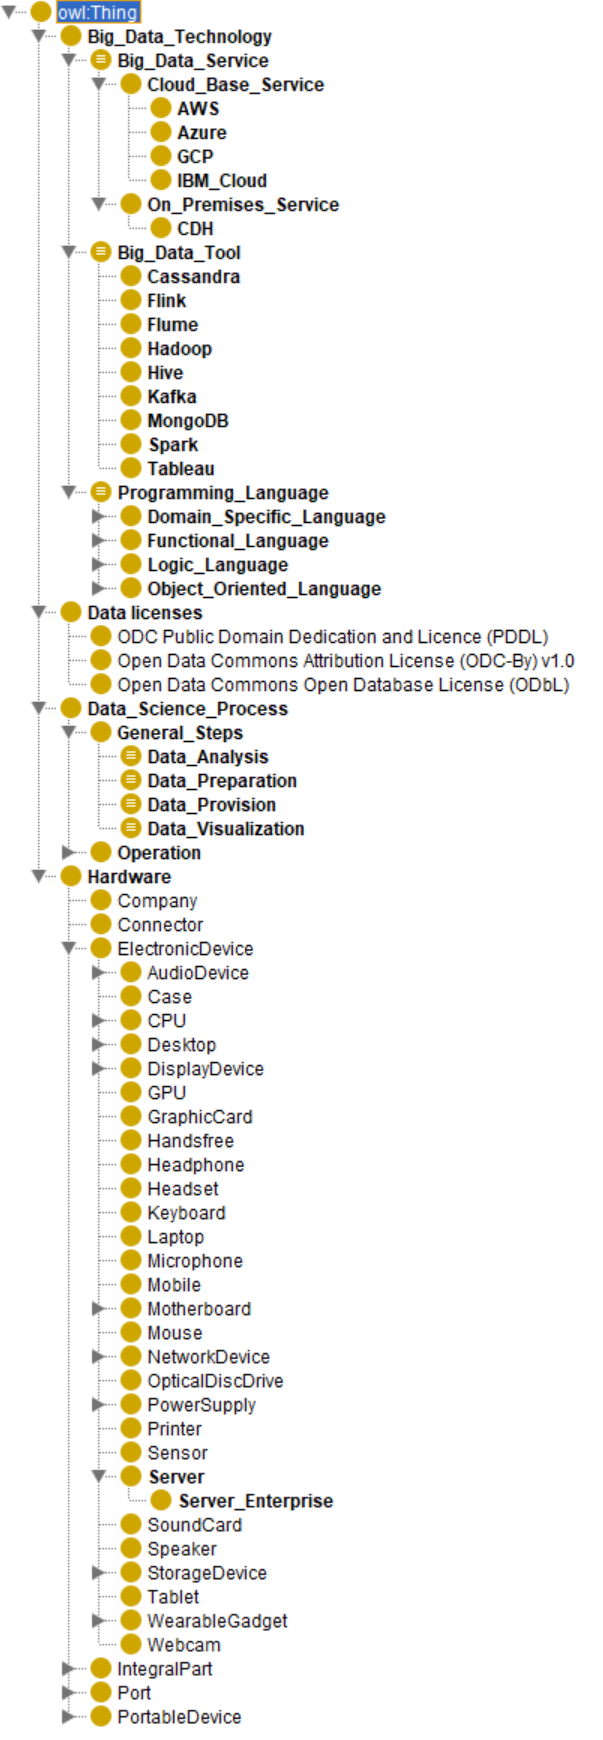
\includegraphics[height=12.5cm]{docs/images/taxonomyWS.PNG}
    \caption{Struttura dell'ontologia BDOnto.}
    \label{fig:classi_bdonto}
\end{figure}
Tutte le classi sono state determinate seguendo un approccio iterativo, cambiando più volte la struttura generale a seconda delle esigenze che nel corso dello svluppo nascevano e secondo ciò che veniva definito all'interno della letteratura.\\

Per facilitare il lettore nella comprensione, ecco un estratto (Figura \ref{fig:owlviz_bdonto}) della gerarchia delle classi creata tramite il plugin \textbf{OWLViz} presente in \textbf{Protégé}.

\begin{figure}[H]
    \centering
    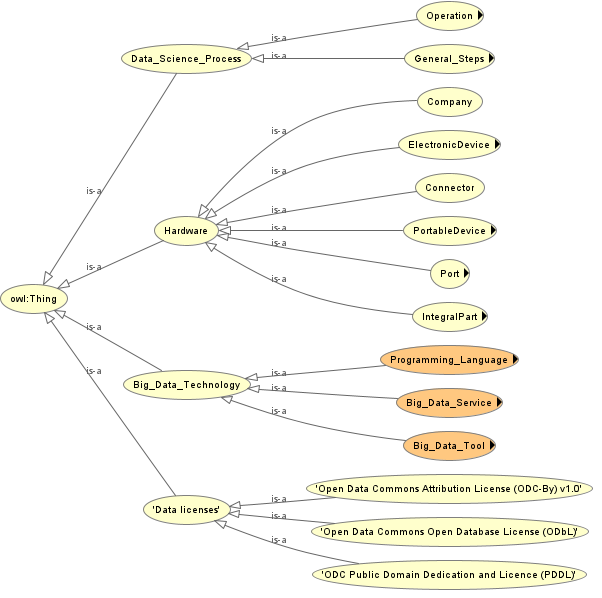
\includegraphics[width=15cm]{docs/images/owlvizBdonto.png}
    \caption{Struttura dell'ontologia BDOnto attraverso \textit{OWLViz}.}
    \label{fig:owlviz_bdonto}
\end{figure}
\newpage
\section{Valutazione delle Object Properties}
Le object properties hanno aiutano a modellare le relazioni e le interconnessioni tra le diverse entità nel dominio, consentendo poi al reasoner di inferire nuove informazioni sulla base di tali relazioni. Inoltre, agevolano la ricerca e l'interrogazione dell'ontologia, consentendo agli utenti di recuperare informazioni specifiche attraverso le connessioni definite. L'analisi del dominio ha permesso, in seguito, di individuare quelle proprietà specifiche che modellano i vincoli tra classi negli individui.\\

Nella figura seguente (Figura \ref*{fig:proprieta_bdonto}) si notano molte proprietà, tante delle quali sono state importate dalle ontologie estese sopra nominate.
\begin{figure}[H]
    \centering
    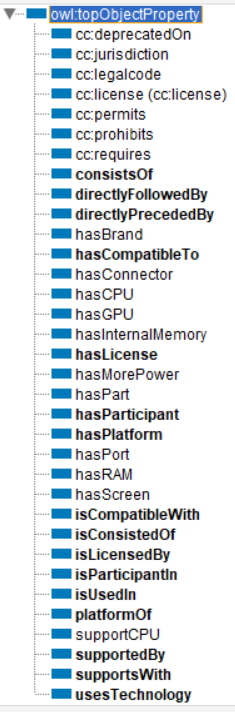
\includegraphics[width=4.2cm]{docs/images/datapropWS.PNG}
    \caption{Object properties dell'ontologia BDOnto. In grassetto le proprietà definite da noi.}
    \label{fig:proprieta_bdonto}
\end{figure}

Per quanto riguarda l'ontologia progettata, ogni proprietà presenta la sua inversa, il che è una buona pratica per consentire la navigazione bidirezionale nell'ontologia.\\

Sono quindi state modellate le seguenti proprietà:
\begin{itemize}
    \item \textbf{consistsOf}: modella le operazioni che possono fare parte di uno specifico step del Data Science Process;
    \item \textbf{isConsistedOf}: proprietà inversa di \textit{consistsOf};
    \item \textbf{directlyFollowedBy}: proprietà \textit{funzionale ed inversa funzionale} che modella l'ordine degli step in un progetto di Data Science;
    \item \textbf{directlyPrecededBy}: proprietà \textit{funzionale ed inversa funzionale} di \textit{directlyFollowedBy};
    \item \textbf{isCompatibleWith}: proprietà \textit{transitiva}, che modella la compatibilità tra due sistemi;
    \item \textbf{hasCompatibleTo}: proprietà \textit{transitivia} ed inversa di \textit{isCompatibleWith};
    \item \textbf{hasLicense}: proprietà \textit{funzionale inversa} che modella la relazione di regolamentazione legale da parte di una licenza su un tool;
    \item \textbf{isLicensedBy}: proprietà inversa di \textit{hasLicense};
    \item \textbf{hasParticipant}: modella la partecipazione di un elemento all'interno di un dato step della Data Science;
    \item \textbf{isParticipantIn}: proprietà inversa di \textit{hasParticipant};
    \item \textbf{supportsWith}: modella il supporto di una certa tecnologia o linguaggio o altro ancora da parte di un dato tool o tecnologia;
    \item \textbf{supportedBy}: proprietà inversa di \textit{supportsWith};
    \item \textbf{usesTechnology}: modella la relazione di impiego di una tecnologia da parte di un'altra tecnologia;
    \item \textbf{isUsedIn}: proprietà inversa di \textit{usesTechnology};
    \item \textbf{hasPlatform}: proprietà \textit{funzionale} modella la compagnia che regola, sviluppa, detiene una tecnologia;
    \item \textbf{platformOf}: proprietà inversa di \textit{hasPlatform}.
\end{itemize}

Qualora ritenevamo avesse senso modellare il concetto di \textit{Dominio} e \textit{Range} all'interno di queste proprietà è stato fatto (in modo tale da facilitare il reasoner), altrimenti è stata lasciata piena libertà di utilizzo (ed evitare 'inaspettate' classificazioni, come suggerito in \cite{Protege_Tutorial}).

\section{Valutazioni delle Data Properties}

Durante l'analisi iniziale, le varie entità presenti non risultavano caratterizzate da valori numerici, quindi non si presentavano \textit{Data Properties}. Questa caratteristica, che rendeva il dominio poco interessante e molto "tassonomico", andava superata. Ci siamo quindi sforzati nel cercare informazioni numeriche per le entità di questo dominio. Dopo diversi tentativi, sono state modellate delle proprietà numeriche per le principali classi della tassonomia, che hanno particolarmente arricchito il progetto. Queste proprietà sono state fondamentali in fase di modellazione di alcune classi di equivalenza. Un esempio, è la classe Big Data Tool è equivalente ad una Big Data Technology che supporta almeno un linguaggio di programmazione, che ha una certa dimensione in MB, ha una certa versione, ecc.\\

Nello specifico sono state modellate le seguenti Data Properties:
\begin{itemize}
    \item \textbf{hasAverageCost}: indica il costo medio (in dollari) di una tecnologia; deve avere un valore maggiore o uguale a 0.0.
    \item \textbf{hasAverageSize}: indica la dimensione media del software (in MB); deve avere un valore maggiore o uguale a 0.0.
    \item \textbf{hasDifficultyLevel}: indica la difficoltà nell'usare una tecnologia; i valori variano da 1 (facile) a 5 (estremamente difficile).
    \item \textbf{hasEndOfSupportDate}: indica la data nella quale una tecnologia smetterà di essere supportata o ha cessato di essere supportata.
    \item \textbf{hasFullName}: indica il nome completo di quella entità.
    \item \textbf{hasLearningCurve}: indica la pendenza della curva di apprendimento di una data tecnologia; i valori variano da 1 (ritmo rapido) a 5 (ritmo estremamente lento).
    \item \textbf{hasStartingDate}: indica la data nella quale l'entità è nata.
    \item \textbf{hasVersion}: indica la versione della tecnologia.
    \item \textbf{hasParadigm}: indica il paradigma di programmazione supportato dal linguaggio (es. imperativo, dichiarativo, orientato agli oggetti).
    \item \textbf{hasLifespan}: indica la durata (in mesi) del supporto a tale tecnologia.
\end{itemize}

Abbiamo modellato i concetti di \textit{Dominio} e \textit{Range} all'interno di queste proprietà solo quando lo abbiamo ritenuto opportuno, seguendo un approccio flessibile.\\

Le ontologie importate portavano con sè un numero considerevole di proprietà quindi qui di seguito vengono mostrate solo alcune delle Data Properties presenti all'interno dell'ontologia:

\begin{figure}[H]
    \centering
    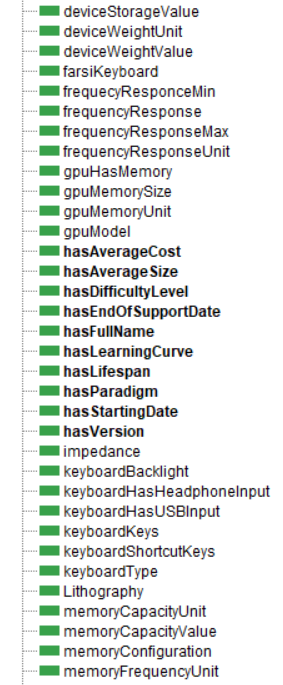
\includegraphics[height=14cm]{docs/images/objpropWS.PNG}
    \caption{Data properties dell'ontologia. In grassetto le proprietà definite da noi.}
    \label{fig:datap_bdonto}
\end{figure}

